\section{The \igh{} locus in \xma}
\label{sec:xma-locus}
	
	The turquoise killifish \igh{} locus shares many features with other characterised teleost loci, including a modified tandem-translocon configuration with intact \vh, \dh, \jh and constant regions (\Cref{fig:nfu-locus-map-b}), a four-exon secreted configuration of \igh{M} (\Cref{fig:nfu-locus-sashimi-a}), an expanded \igh{D} constant region with tandem \cd{}-exon block repeats (\Cref{fig:nfu-locus-sashimi-b,fig:nfu-locus-map-b},), a conserved RSS structure (\Cref{fig:nfu-rss-seqlogo-all}), and a chimeric \cm{1} in \igh{D} (\Cref{fig:nfu-locus-sashimi-b}). However, it also exhibits many ideosyncratic features that differ from those observed in most characterised teleost loci, including an unusually small number of \vh segments (\Cref{fig:nfu-vh-families} and \Cref{tab:teleost-vh-counts}), a four-exon \cm{1}-\cm{2}-TM1-TM2 configuration of transmembrane \igh{M} (\Cref{fig:nfu-locus-sashimi-a}), an inverted sublocus present in antisense (\Cref{fig:nfu-locus-map-b}), and a complete absence of \igh{Z}.
	
Many of these peculiarities, including the unusual \igh{M-TM} splicing pattern, inverted sublocus, and lack of \igh{Z}, are shared with the \igh{} locus of medaka (\textit{Oryzias latipes}), which is the closest relative of \textit{Nothobranchius furzeri} to have its immunoglobulin heavy chain locus characterised prior to this study \parencite{magadan2011medaka}. Given the close relationship between the two species, the shared unusual features of their \igh{} loci suggested a common origin of these traits  in the common ancestor of both species. If this hypothesis were correct, one would expect \igh{Z} to also be absent in any other descendents of this common ancestor, including other cyprinodontiform species.

To investigate this hypothesis further, I performed a complete characterisation of the \igh{} locus in the platyfish \textit{Xiphophorus maculatus}, another cyprinodontiform species that has seen widespread use as a model organism \parencite{schartl2013platyfish}. Surprisingly, the \Xma locus shared none of the unusual features shared between the turquoise-killifish and medaka loci, strongly suggesting independent loss of \igh{Z} in both groups and implying a high level of volatility in \igh{} locus structure within the Atherinomorpha.

\subsection{Overall structure}
\label{sec:xma-locus-structure}
	
As was the case with the \Nfu \igh{} locus, candidate genome scaffolds from the most recent \xma genome assembly (Genbank accession GCA\_002775205.2) were identified by alignment to \igh{} gene segments from zebrafish, stickleback and medaka, supplemented in this case with segments from the newly-characterised \Nfu locus itself. In contrast to the more fragmented results in \Nfu, this process identified a single sequence region on one chromosome of the \Xma locus, which was extracted and characterised as described for the assembled \Nfu locus (\Cref{sec:nfu-locus}) without the need for further sequencing or assembly.

The \Xma \igh{} locus so identified occupies roughly \kb{293} on chromosome 16 (scaffold NC\_036458.1; \Cref{fig:xma-locus-map-a}). Unlike in turquoise killifish and medaka, all identified gene segments share a common orientation; no evidence of a second sublocus in antisense could be identified. In stark contrast with both killifish and medaka, the single ``sublocus" comprising \Xma \igh{} contains not one but two \igh{Z} constant regions, along with a hugely extended V-region extending over almost \kb{250} and containing more than 120 \vh-segments. This enormous \vh-diversity greatly exceeds that of any characterised teleost \igh{} locus except perhaps that of rainbow trout \parencite{bengten2015fishantibodies}, while the presence of multiple \igh{Z} constant regions without intervening \igh{M} or \igh{D} is also highly unusual \parencite{fillatreau2013astonishing}. 

Even cursory examination of the \Xma \igh{} locus is therefore sufficient to reveal a unique and highly interesting structure with many unexpected differences from both turquoise killifish and medaka (\Cref{fig:species-tree-small}, columns 1-5). In particular, since \Xma is more closely related to \Nfu than either is to medaka, the presence of \igh{Z} in the former strongly suggests at least two independent loss events in the Atherinomorpha, indicating an unexpected level of volatility in the evolution of this important isotype.
 
	\begin{figure}
	\centering
	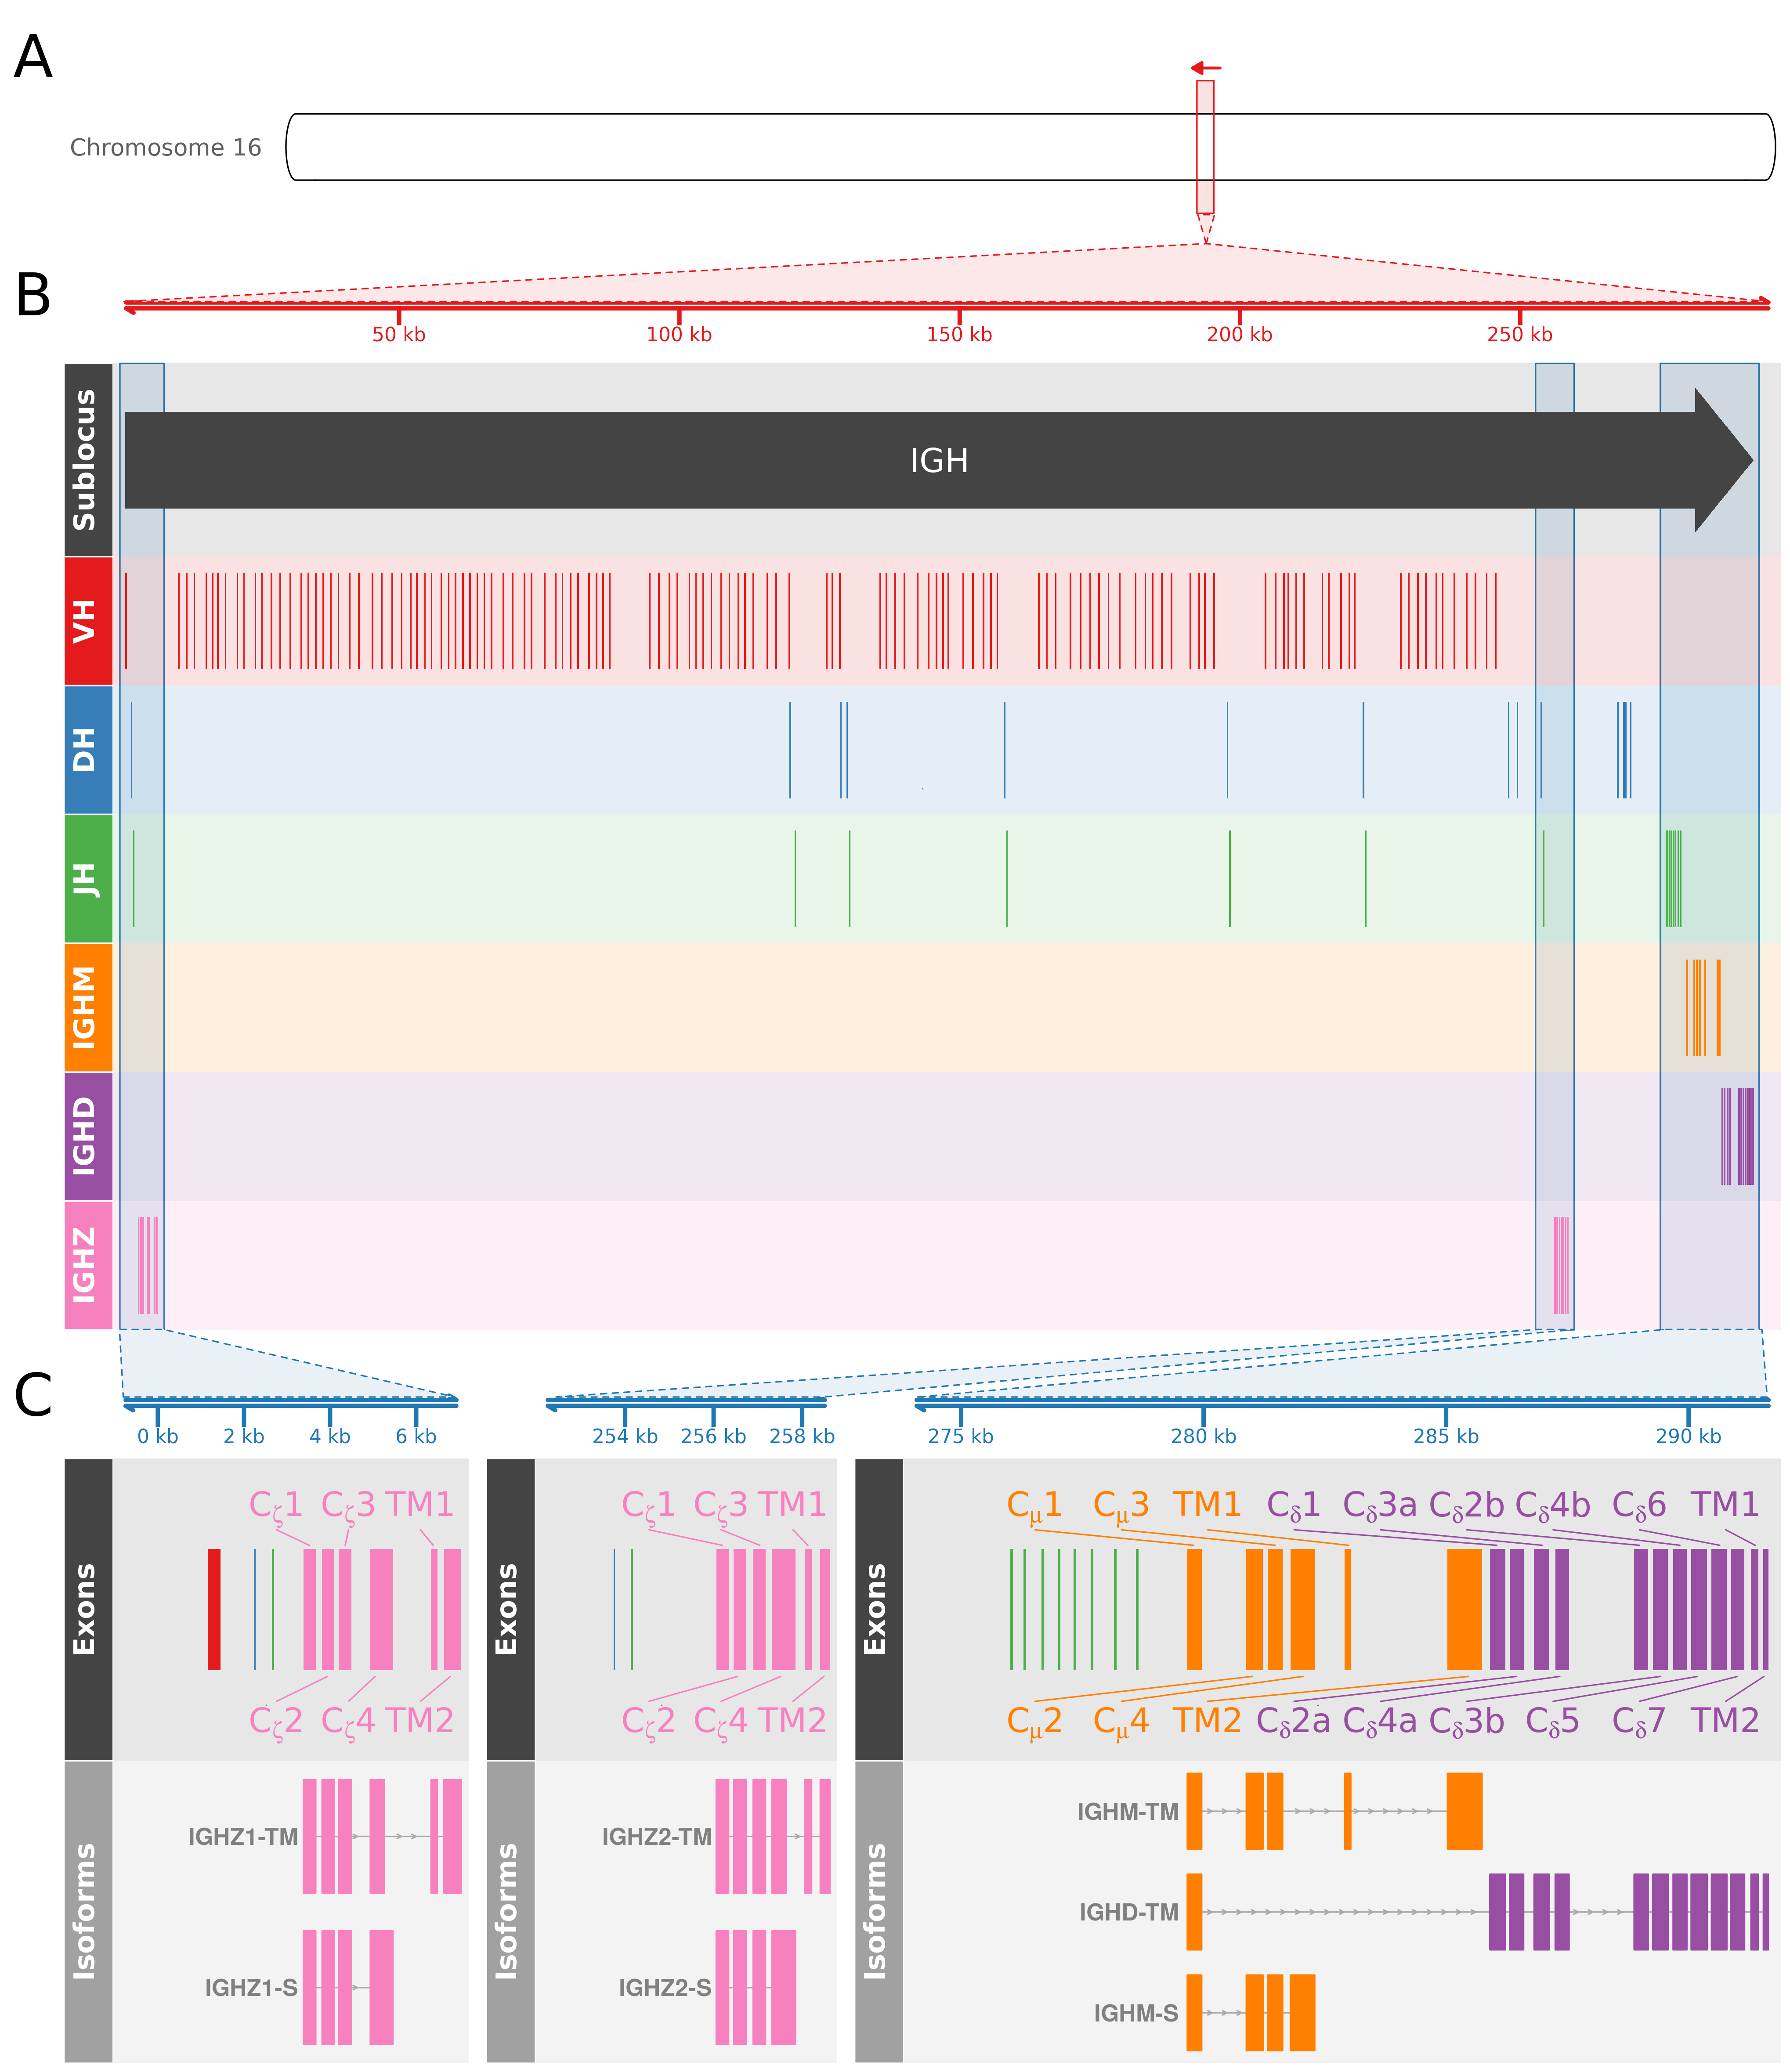
\includegraphics[width=\textwidth]{_Figures/png/xma-new-locus-map}
	\caption[The immunoglobulin heavy chain (\textit{IGH}) locus in \textit{}]{\textbf{The immunoglobulin heavy chain (\textit{IGH}) locus in \textit{Xiphophorus maculatus}:} (A) Position of the \textit{IGH} locus on chromosome (group) 16 of the \Xma genome. (B) Arrangement of \vh, \dh, \jh and constant-region gene segments on the \Xma \igh{} locus. (C) Detailed map of the \igh{Z1}, \igh{Z2} and \igh{M/D} constant regions, indicating the position and identity of the constant-region exons and the exon composition of expressed \igh{} isoforms in \Xma. Note change of orientation between subfigures (A) and (B-C).}
	\begin{subfigure}{0em}
        \phantomsubcaption{}
        \label{fig:xma-locus-map-a}
    \end{subfigure}
    \begin{subfigure}{0em}
        \phantomsubcaption{}
        \label{fig:xma-locus-map-b}
    \end{subfigure}
    \begin{subfigure}{0em}
        \phantomsubcaption{}
        \label{fig:xma-locus-map-c}
    \end{subfigure}
	\label{fig:xma-locus-map}
\end{figure} % TODO: Fix to remove IGHZ2-S

\begin{figure}
\centering
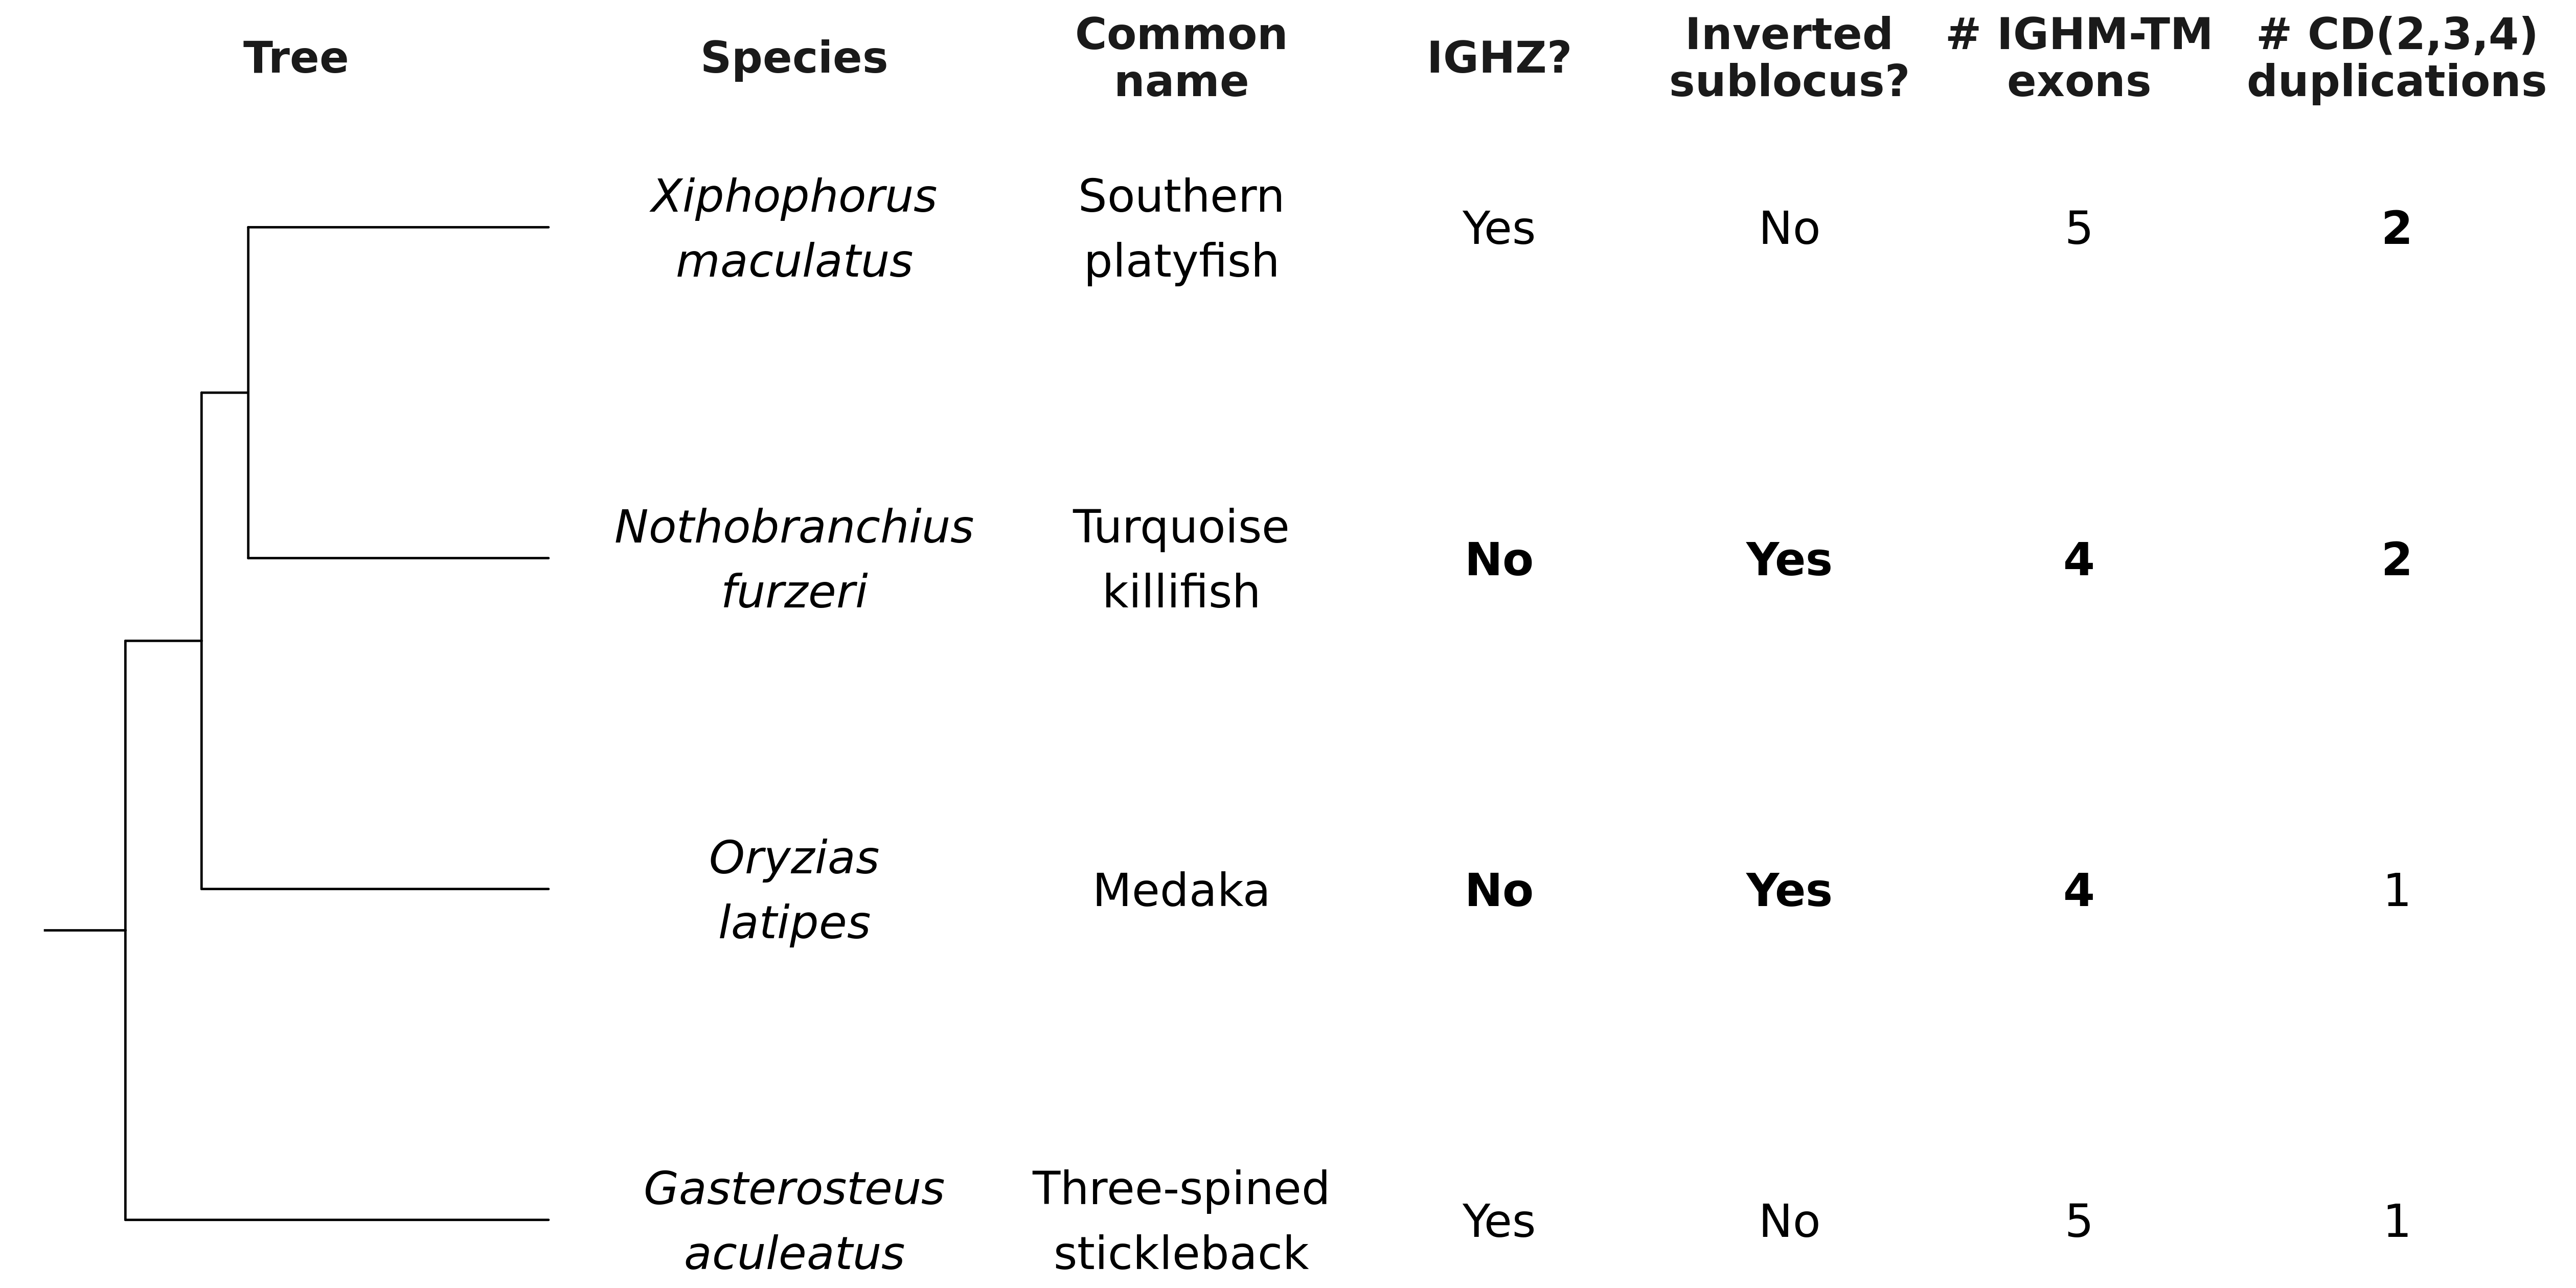
\includegraphics[width=\textwidth]{_Figures/png/species-tree-small}
\vspace{0.5em}
\caption[Summary of important \igh{} phenotypes in killifish, platyfish, and medaka]{\textbf{Summary of important \igh{} phenotypes in killifish, platyfish, and medaka:} Cladogram of the evolutionary relationship between southern platyfish (\xma), turquoise killifish (\nfu) and medaka (\species{Oryzias}{latipes}), with three-spined stickleback (\species{Gasterosteus}{aculeatus}) as an outgroup. The state of various \igh{} phenotypes of interest are annotated to the right of the tree; states deviating from the expected teleost configuration are in bold.}
\label{fig:species-tree-small}
\end{figure}
	
\subsection{Constant regions}
\label{sec:xma-locus-constant}
	
As discussed briefly in \Cref{sec:xma-locus-structure}, the \Xma \igh{} locus contains two distinct \igh{Z} constant regions: one in the usual position immediately preceding the \igh{M}-associated D- and J-regions, the other, unexpectedly, at the far 5'-extremity of the locus (\Cref{fig:xma-locus-map-b}). Both \igh{Z} constant regions occupy the expected configuration, with four \cz{} exons, two transmembrane exons, and a secretory tail (\Cref{fig:xma-locus-map-c}, \Cref{tab:xma-ch-coords}). However, in contrast to the duplicate constant regions in \Nfu, the two \igh{Z} constant regions in \Xma are quite distinct from each other in sequence, with an average of only \pc{64} nucleotide and \pc{48} amino-acid sequence identity between corresponding \cz{} exons (\Cref{fig:xma-cz-aln}, \Cref{tab:xma-cz-aln}). This unexpectedly high level of sequence divergence suggests a relatively ancient duplication event, and raises the possibility that the lineage giving rise to \Nfu may have lost not one, but two distinct \igh{Z} constant regions.
	
\begin{table}
	\centering
	\caption[Sequence similarity between \igh{Z} constant-regions in \Xma]{\textbf{Sequence similarity between \igh{Z} constant-regions in \Xma:} Percentage sequence identities of pairwise Needleman-Wunsch global alignments between nucleotide (NT) or amino-acid (AA) sequences of corresponding \cz{} exons from the two \igh{Z} constant regions of \Xma \textit{IGH}.}
	% latex table generated in R 3.5.2 by xtable 1.8-3 package
% Tue Jan  8 14:15:22 2019
\begin{tabular}{llrr}
  \toprule Isotype & Exon & NT & AA \\ 
  \midrule Z & 1 & 59.14 & 44.57 \\ 
  Z & 2 & 63.93 & 53.41 \\ 
  Z & 3 & 66.19 & 43.48 \\ 
  Z & 4 & 65.15 & 50.49 \\ 
   \bottomrule \end{tabular}

	\label{tab:xma-cz-aln}
\end{table}

While the state of \igh{Z} constant regions differs markedly between \Xma and \Nfu, the configurations of the \igh{M} and \igh{D} constant regions of the two species are quite similar, with a {\cm{1}-\cm{2}-\cm{3}-\cm{4}-TM1-TM2} configuration for \igh{M} and a {\cd{1}-(\cd{2}-\cd{3}-\cd{4})$_2$-\cd{5}-\cd{6}-\cd{7}-TM1-TM2} configuration for \igh{D} (\Cref{fig:xma-locus-map-b,fig:xma-locus-map-c}, \Cref{tab:xma-ch-coords}). In the \Xma locus, these constant regions and \igh{Z1} adopt the standard configuration seen in comparatively simple teleost \igh{} loci like those of zebrafish and fugu, with a {\vh-\dh-\jh-\textbf{CZ}-\dh-\jh-\textbaf{CM}-\textbf{CD}} arrangement that allows the choice between \igh{Z} and \igh{M/D} usage to be made via the choice of \dh segment during VDJ-recombination. However, whether such a mechanism is also responsible for the choice between these constant regions and \igh{Z1}, which lies more than \kb{200} away and upstream of the great majority of \vh segments in the locus (\Cref{sec:xma-locus-variable}) is questionable.

In order to investigate the expressed isoforms present in \Xma, published RNA-sequencing reads from various platyfish tissues (BioProject accession PRJNA420092, all libraries). were aligned together to the \igh{Z} and \igh{M/D} constant regions with \program{STAR}. The results indicate the expected six-exon transmembrane configuration in both \igh{Z1} and \igh{Z2}, as well as a secretory form of \igh{Z1} comprising \cz{1} to \cz{4} plus a \bp{23} secretory tail formed by a transcriptional run-on event from \cz{4} (\Cref{fig:xma-locus-sashimi-z1,fig:xma-locus-sashimi-z2}). However, while an in-frame secretory tail of similar length (\bp{20}) can be found in \igh{Z2}, it does not appear to be expressed in the read sets analysed here, indicating that \igh{Z2} may only be expressed in transmembrane form in the individuals sampled (\Cref{fig:xma-locus-sashimi-z2}).

Meanwhile, the results for \igh{D} (\Cref{fig:xma-locus-sashimi-d}) indicate a similar configuration to that observed in turquoise killifish, with a chimeric \cm{1} followed by 10 \cd{} exons and two transmembrane exons; as in \Nfu, neither a dedicated \igh{D} secretory exon nor a post-\cd{7} secretory tail was identified, suggesting that \igh{D} may be produced solely in transmembrane form in this species. Secretory \igh{M} (\igh{M-S}) was also found to occupy the same four-exon configuration seen in turquoise killifish and elsewhere. However, the configuration observed for transmembrane \igh{M} (\igh{M-TM}) did not correspond to the four-exon structure shared between turquoise killifish and medaka (\Cref{fig:nfu-locus-sashimi-a}); rather, \igh{M-TM} in \Xma occupies the five-exon configuration seen in most characterised teleosts (\Cref{fig:teleost-igm-exons-d}). This surprising difference indicates that two different splice configurations of \igh{M-TM} persist in the cyprinodontiform lineage, and raises the question of what, if any, functional difference arises from the presence or absence of \cm{3} in transmembrane \igh{M} in different species. However, it remains unclear whether this pattern of exon usage (\Cref{fig:species-tree-small}) is the result of independent changes in medaka and turquoise killifish or of a reversion in \Xma to the primitive teleost configuration.
	
\begin{figure}
	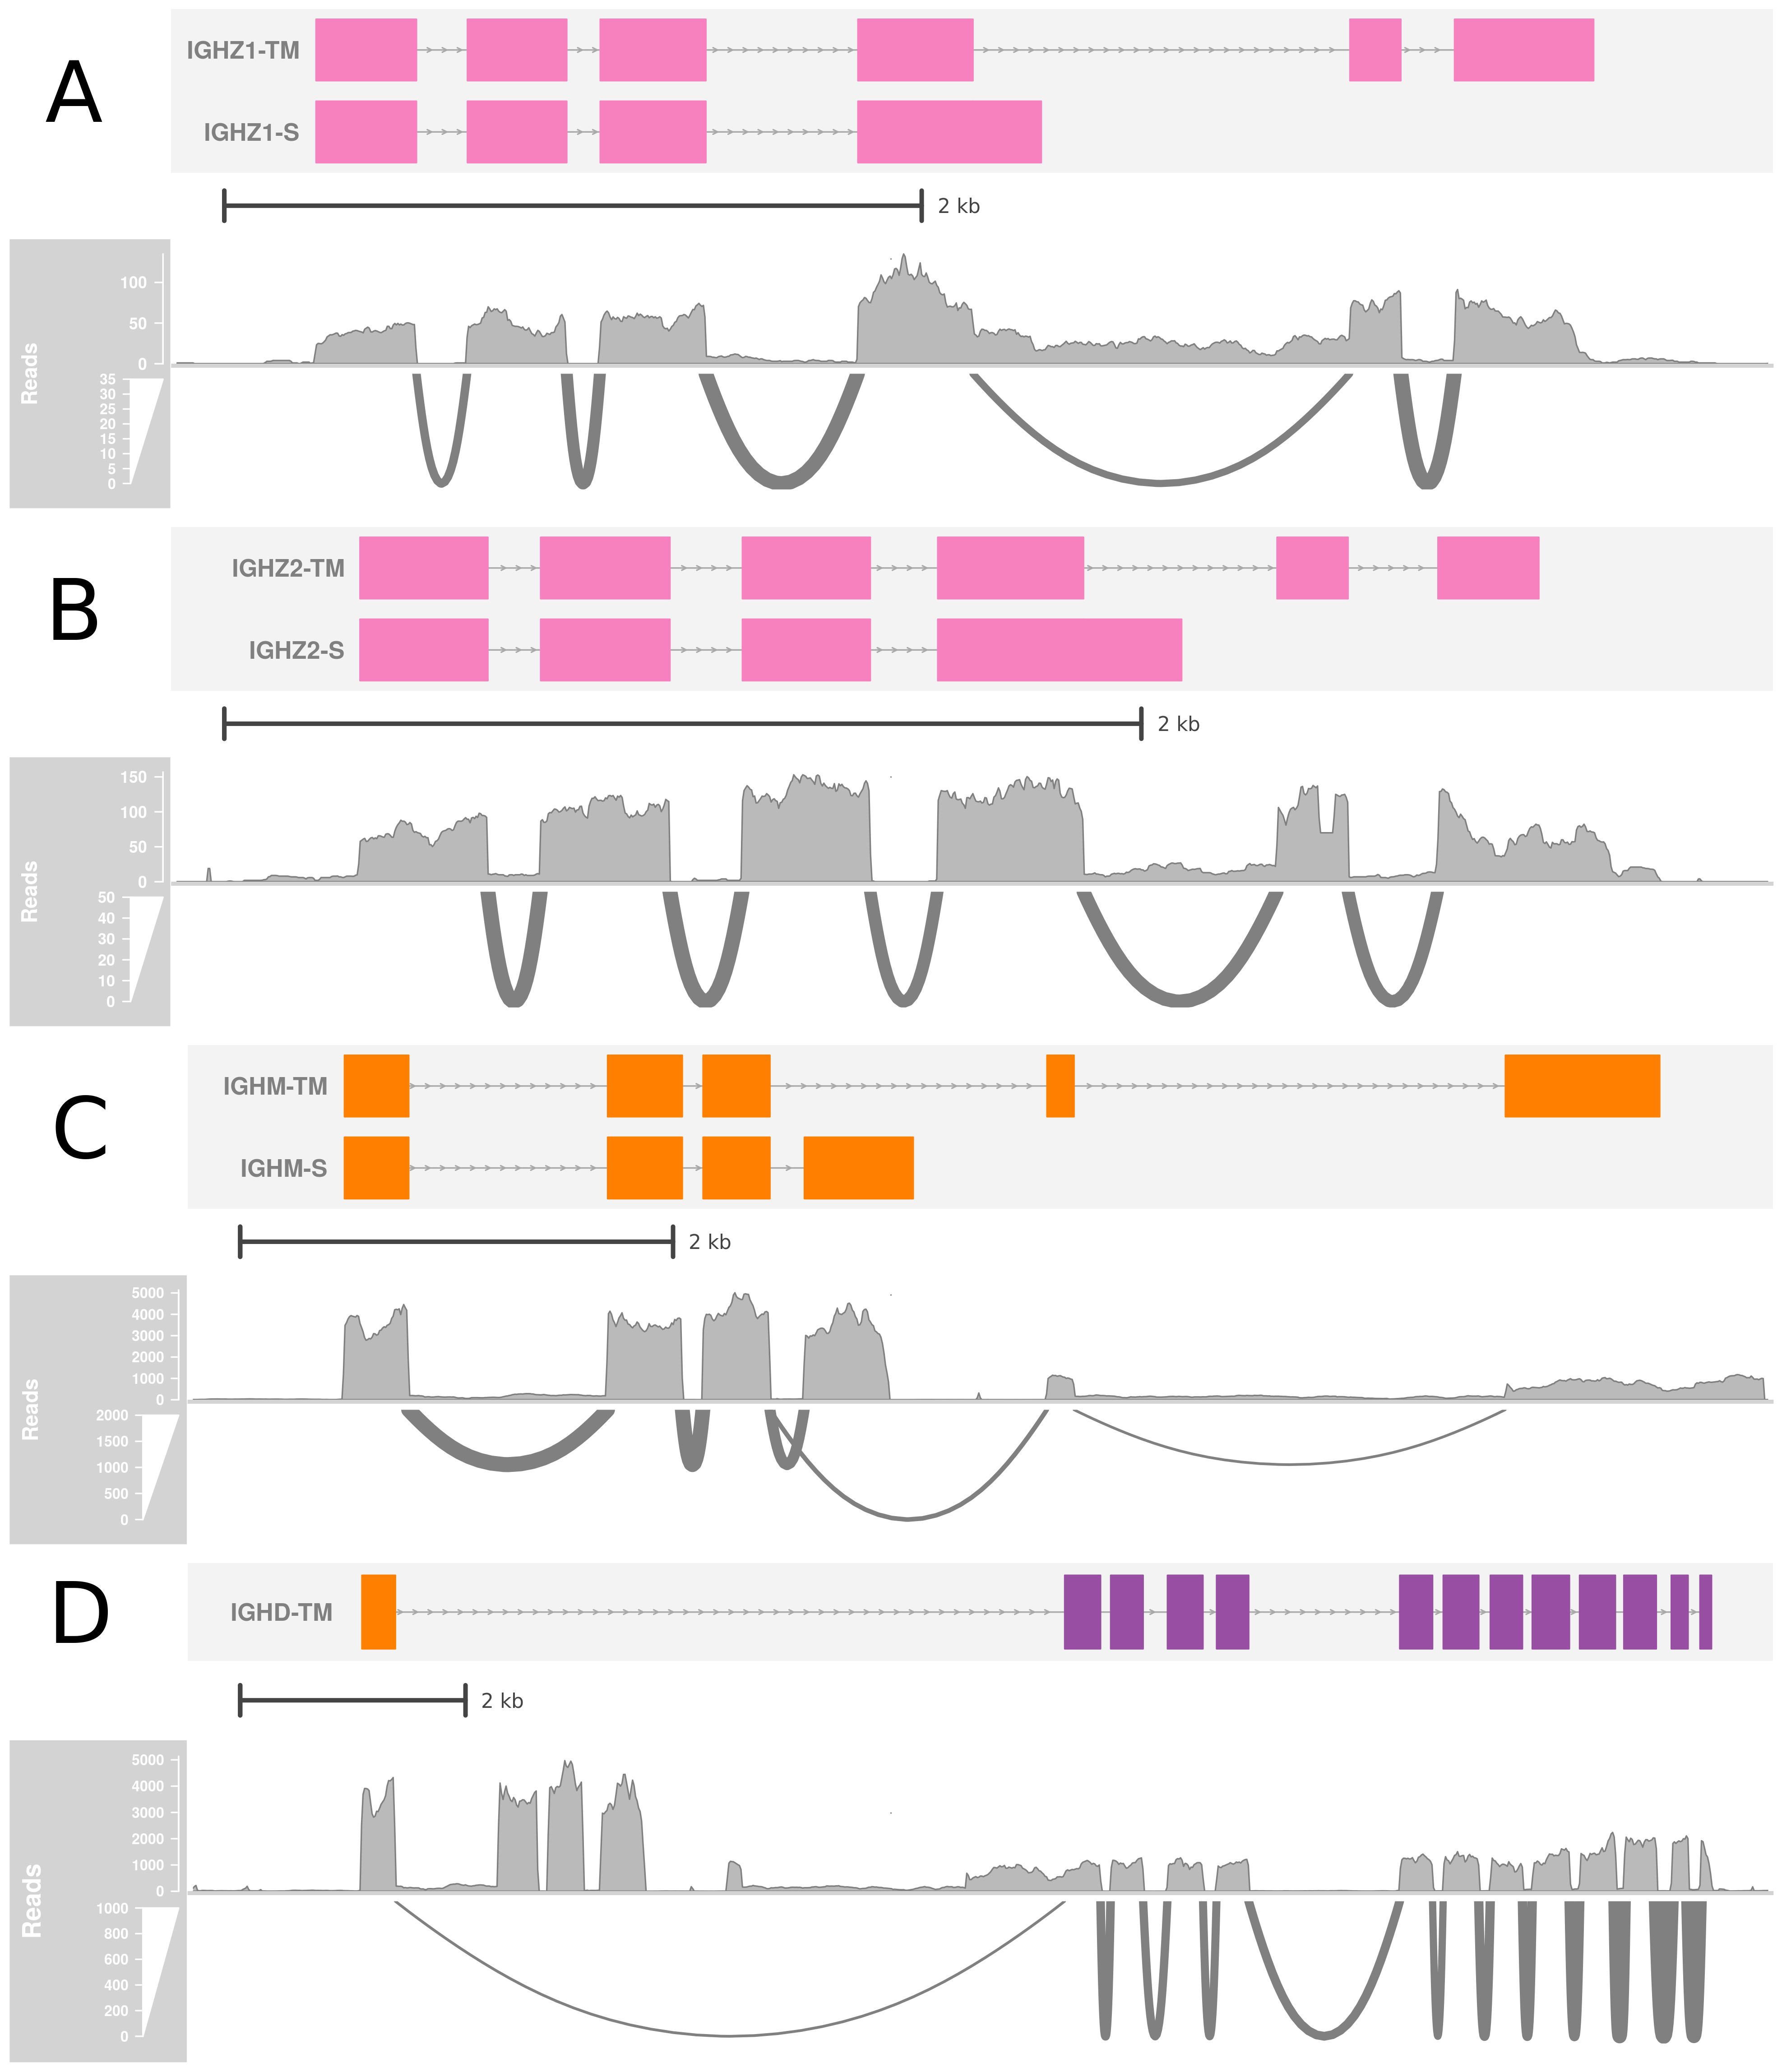
\includegraphics[width=\textwidth]{_Figures/png/xma-new-locus-sashimi}
	    \begin{subfigure}{0em}
        \phantomsubcaption{}
        \label{fig:xma-locus-sashimi-z1}
    \end{subfigure}
    \begin{subfigure}{0em}
        \phantomsubcaption{}
        \label{fig:xma-locus-sashimi-z2}
    \end{subfigure}
	\begin{subfigure}{0em}
        \phantomsubcaption{}
        \label{fig:xma-locus-sashimi-m}
    \end{subfigure}
    \begin{subfigure}{0em}
        \phantomsubcaption{}
        \label{fig:xma-locus-sashimi-d}
    \end{subfigure}
	\caption[Constant-region isoforms in \Xma]{\textbf{Constant-region isoforms in \Xma:} Coverage and sashimi plots of STAR-aligned RNA-seq reads from \Xma samples, demonstrating the splicing behaviour of \igh{} constant-region isoforms. (A) \igh{Z1} exon splicing, showing alternative use of the \cz{4}/TM1 splice junction and the post-\cz{4} secretory tail; (B) \igh{Z2} exon splicing; (C) IGHM exon splicing, showing alternative splicing patterns of IGHM-TM and IGHM-S; (D) IGHD exon splicing, including splicing of \cm{1} to \cd{1}.}
	\label{fig:xma-locus-sashimi}
	\end{figure}

	
\subsection{Variable regions}
\label{sec:xma-locus-variable}

In total, 125 \vh segments, 14 \dh segments and 15 \jh segments were identified in the \Xma IGH locus (\Cref{fig:xma-locus-map-b}). Of these, exactly one \vh (\igh{V01-01}), \dh (\igh{DZ01}) and \jh (\igh{JZ01}) lie upstream of the \igh{Z1} constant region, indicating that the variable-region sequence diversity available to this isotype is limited to a single VDJ combination. In contrast, the variable region between the end of \igh{Z1} and the start of \igh{Z2} is highly expanded, with 124 tightly-clustered \vh segments -- more than five times the total number seen in \Nfu, and more than seven times the number in the largest \Nfu sublocus. Of these 124 \vh segments, 106 (\pc{86}) are apparently functional, with the remainder pseudogenised by a variety of frameshift mutations, nonsense mutations, or truncation events (\Cref{tab:xma-vh-coords-1,tab:xma-vh-coords-2,tab:xma-vh-coords-3,tab:xma-vh-coords-4,tab:xma-vh-coords-5}); it remains to be seen whether \igh{V01-01} is also capable of recombining with \dh segments downstream of the \igh{Z1} constant region, and so constitutes part of the range of VDJ combinations available to the other constant regions. The \vh sequences in the \Xma locus are much more tightly packed than in the \Nfu locus, consistent with a lower overall prevalence of repetitive regions (21\%) in the \Xma genome \parencite{yuan2018repeats}.
	
In total, the \vh regions in \Xma \textit{IGH} fall into 23 families, of which eight contain multiple segments (\Cref{fig:xma-vh-families-tree,fig:xma-vh-families-map}); strikingly, the single \vh segment serving IGHZ (\igh{V01-01}) represents a separate family which is distinct from any other segment in the locus. To further investigate the evolutionary history of these families, the \vh segments from both the \Xma and \Nfu \igh{} loci were aligned together with \program{PRANK}, and the resulting alignment was used to construct a phylogenetic tree with \program{RAxML} \parencite{stamatakis2014raxml8,stamatakis2005raxml3,stamatakis2006raxml6}; the resulting tree (\Cref{fig:nfu-xma-vh-tree-nt}) revealed a clear interrelationship between the largest families in both loci (\Xma V02 and \Nfu V1), with a similar relationship observed for the second-largest families (\Xma V03 and \Nfu V2). 
In accordance with the close sequence relationship noted in \Cref{sec:nfu-locus-variable}, \Nfu V4 falls comfortably within the V03/V2 subtree, supporting its status as a pseudogenised subfamily of \Nfu V2.
		
In addition to its highly expanded \vh region, the variable region of the \Xma locus is unusual in the arrangement of its \dh and \jh segments (\Cref{tab:xma-dh-coords-seg,tab:xma-jh-coords-seg}): in addition to the relatively densely-packed blocks of four \dh and eight \jh regions between \igh{Z1} and \igh{M}, and the smaller groups of three \dh segments and one \jh segment between the last \vh segment and \igh{Z1}, small numbers of \dh and \jh segments are interspersed between blocks of \vh segments in the extended V-region between \igh{Z1} and \igh{Z2} (\Cref{fig:xma-locus-map-b}). Many of these segments are arranged such that groups of one or two \dh segments are closely associated with a single \jh segment, raising the possibility of a more cluster-like behaviour in which each VDJ group acts as a distinct recombination unit. However, the presence of larger D- and J-regions more closely upstream of the constant regions suggests a more conventional translocon behaviour; it remains to be seen which of these traditional models of antigen-receptor structure more closely matches the \textit{in vivo} recombination behaviour of this locus.
		
Finally, as is the case with \Nfu, the recombination signal sequences (RSSs) in \Xma IGH correspond closely to the standard expectations across the vertebrates, with the expected heptamer and nonamer consensus sequences and spacer length distributions (\Cref{fig:xma-rss-seqlogo-all,fig:xma-rss-seqlogo-sep}, 97.6\% of RSS spacers within \bp{1} of the expected conserved length).	

	\begin{figure}
		\begin{subfigure}{0em}
        \phantomsubcaption{}
        \label{fig:xma-rss-seqlogo-all-heptamer}
    \end{subfigure}
    \begin{subfigure}{0em}
        \phantomsubcaption{}
        \label{fig:xma-rss-seqlogo-all-spacer}
    \end{subfigure}
    \begin{subfigure}{0em}
        \phantomsubcaption{}
        \label{fig:xma-rss-seqlogo-all-nonamer}
    \end{subfigure}
	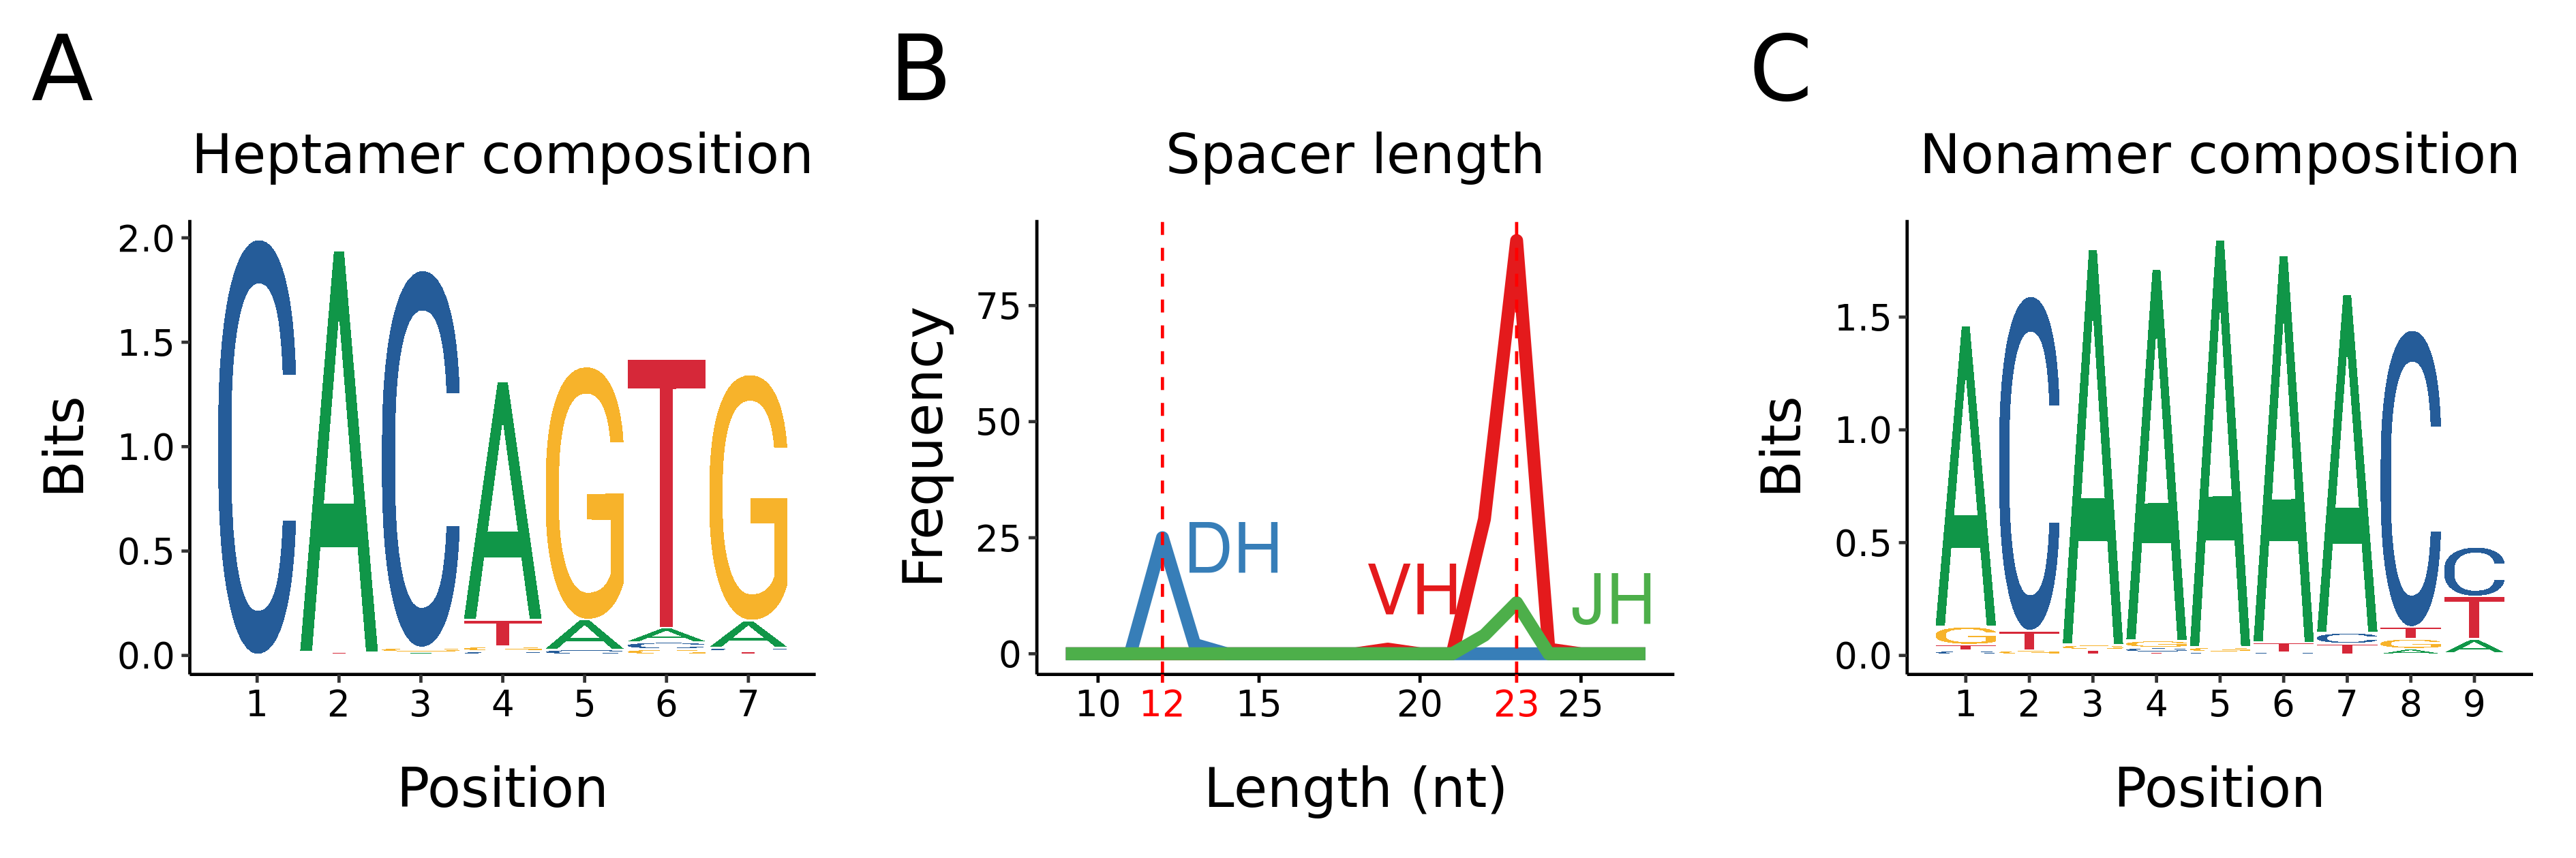
\includegraphics[width=\textwidth]{_Figures/png/xma-new-rss-seqlogo-all}
	\caption[Recombination signal sequences in the \Xma \textit{IGH} locus]{\textbf{Recombination signal sequences in the \Xma \textit{IGH} locus:} (A) Sequence composition of conserved heptamer sequences across all \Xma heavy-chain RSSs; (B) length distribution of unconserved spacer sequences in \Xma heavy-chain RSSs; (C) sequence composition of conserved heptamer sequences across all \Xma heavy-chain RSSs.}
	\label{fig:xma-rss-seqlogo-all}
	\vspace{1em}
	\end{figure}

	
	\begin{figure}
	\centering
	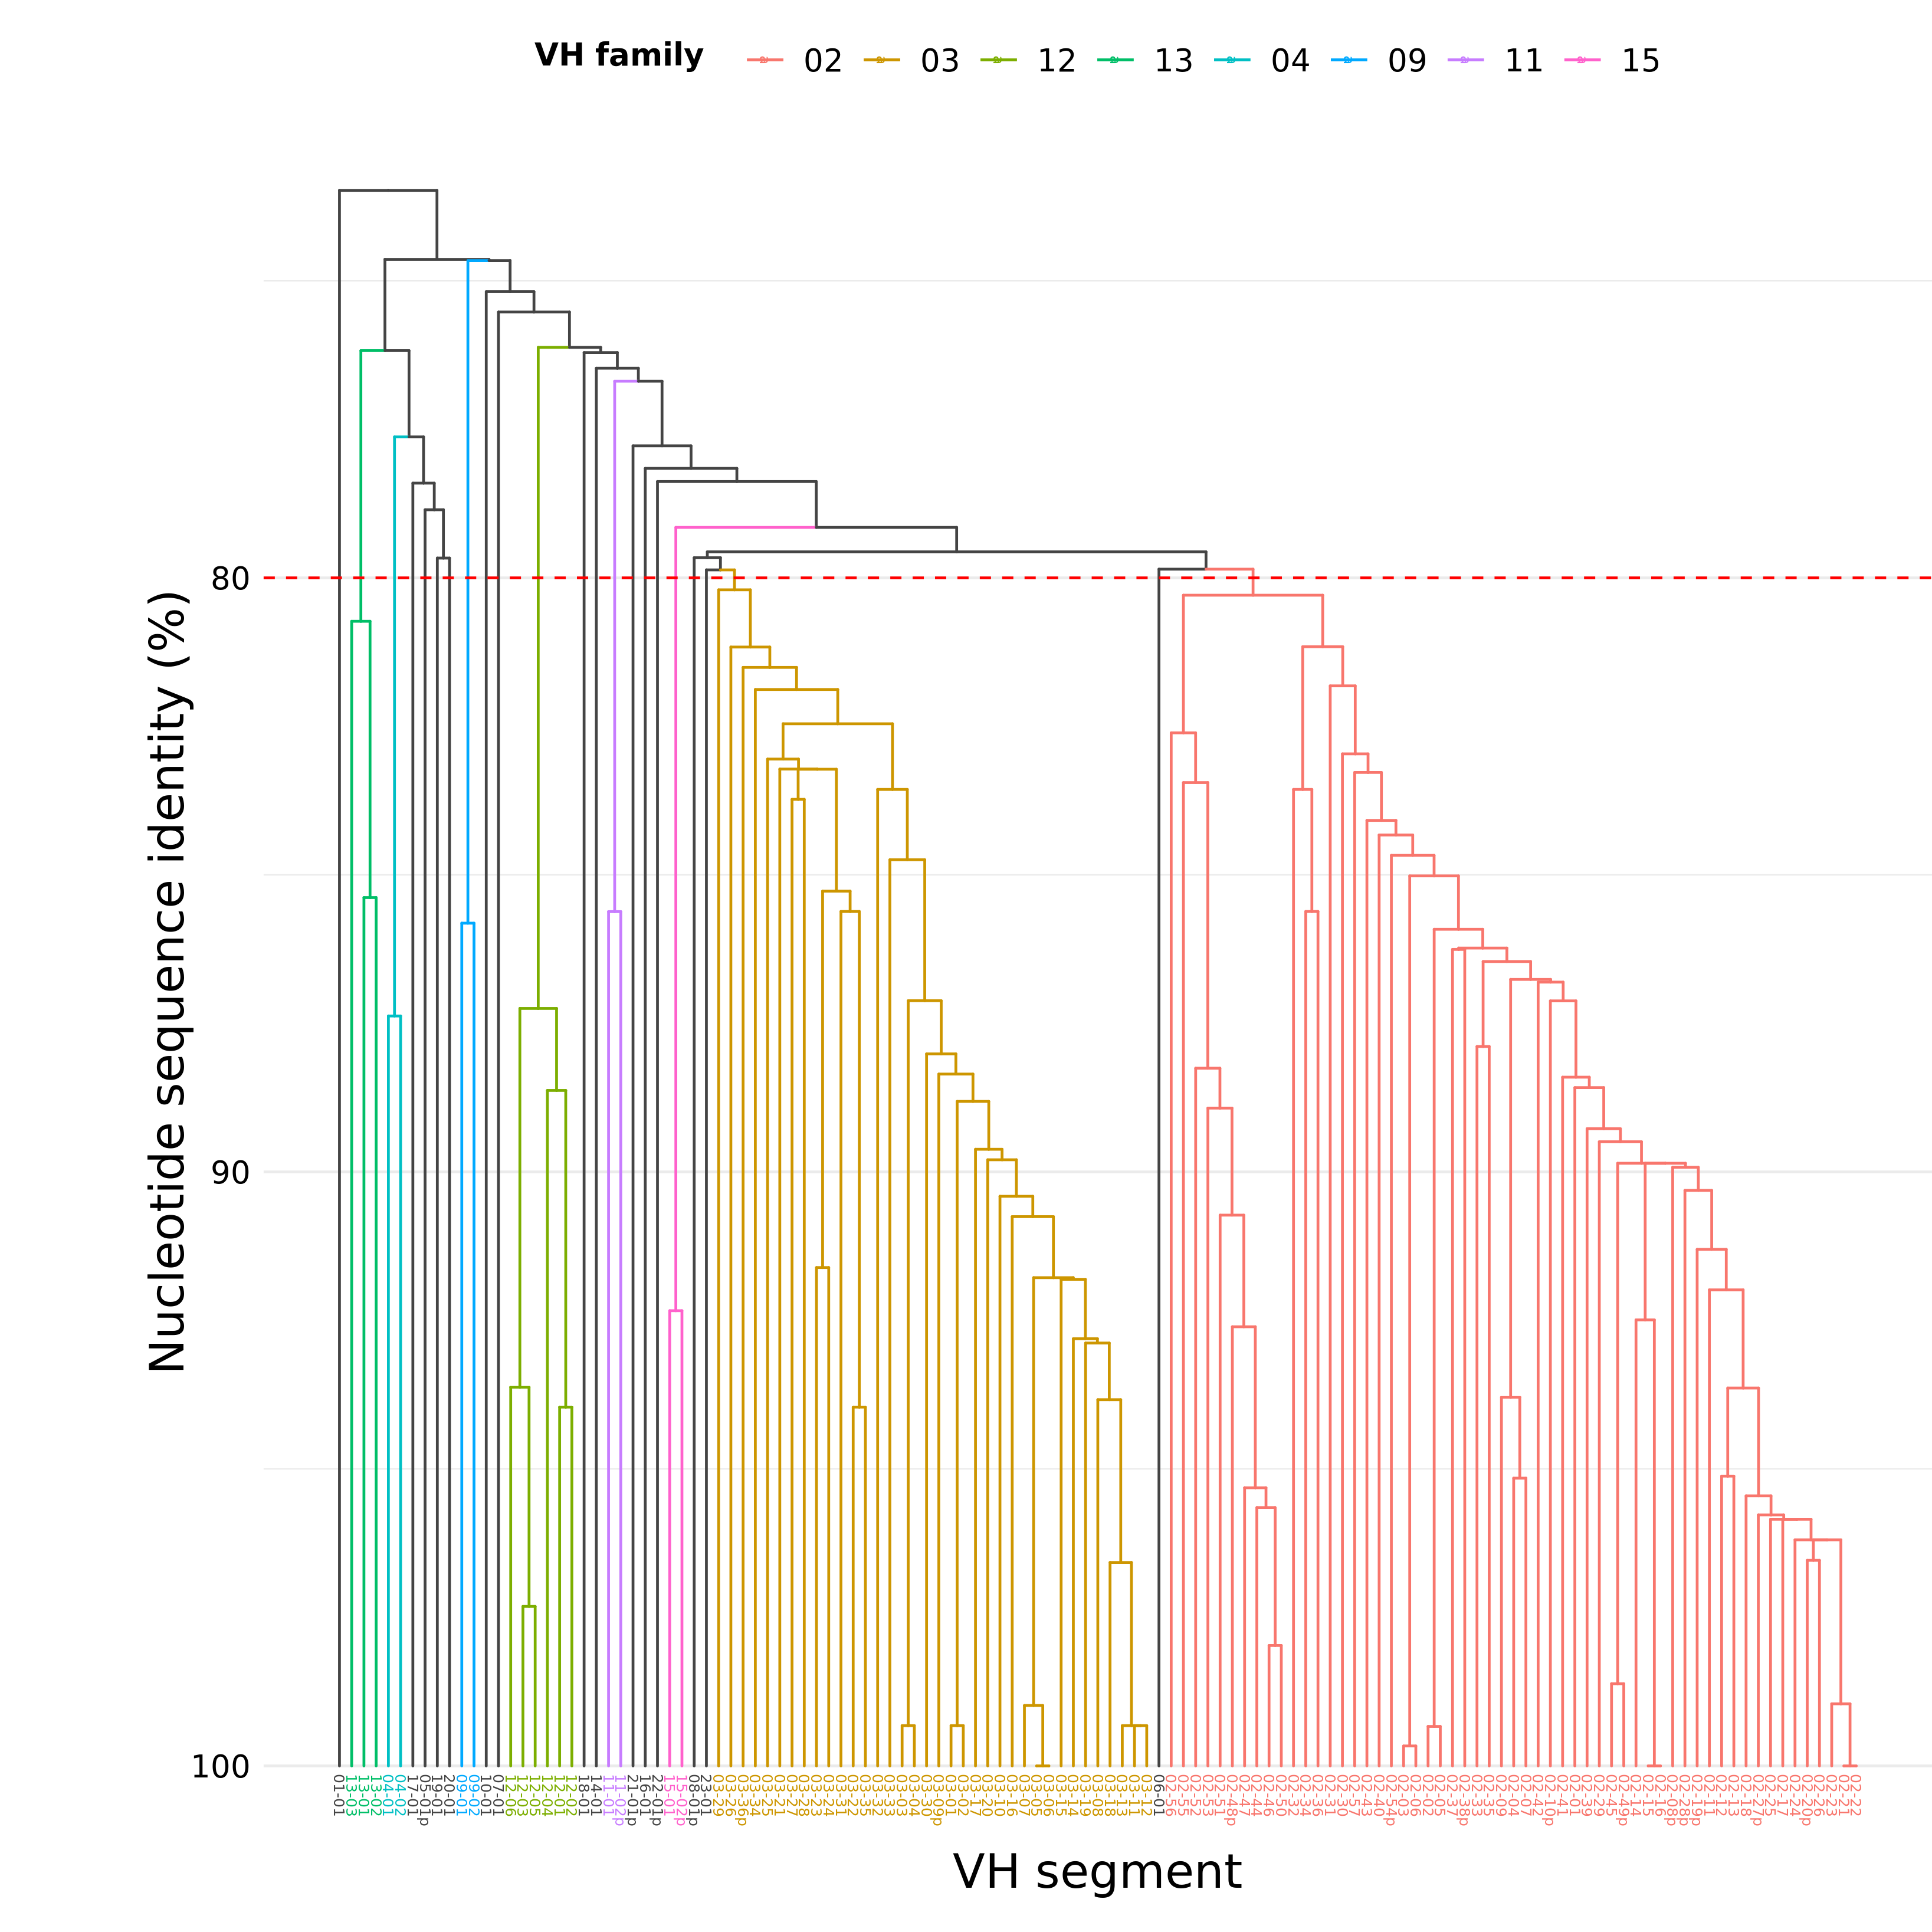
\includegraphics[width=\textwidth]{_Figures/png/xma-vh-families-tree}
	\caption[Dendrogram of \vh families in the in \Xma \textit{IgH} locus]{\textbf{Dendrogram of \vh families in the in \Xma (\textit{IgH}) locus:} Dendrogram of sequence similarity of \vh segments in the \Xma locus, arranged by single-linkage clustering on nucleotide sequence identity. The red line indicates the 80\% cutoff point for family assignment, while branch colour indicates family membership:  \vh families containing multiple segments are uniquely coloured, while single-segment families are in grey.}
	\label{fig:xma-vh-families-tree}
	\end{figure}
		
	\begin{figure}
	\centering
	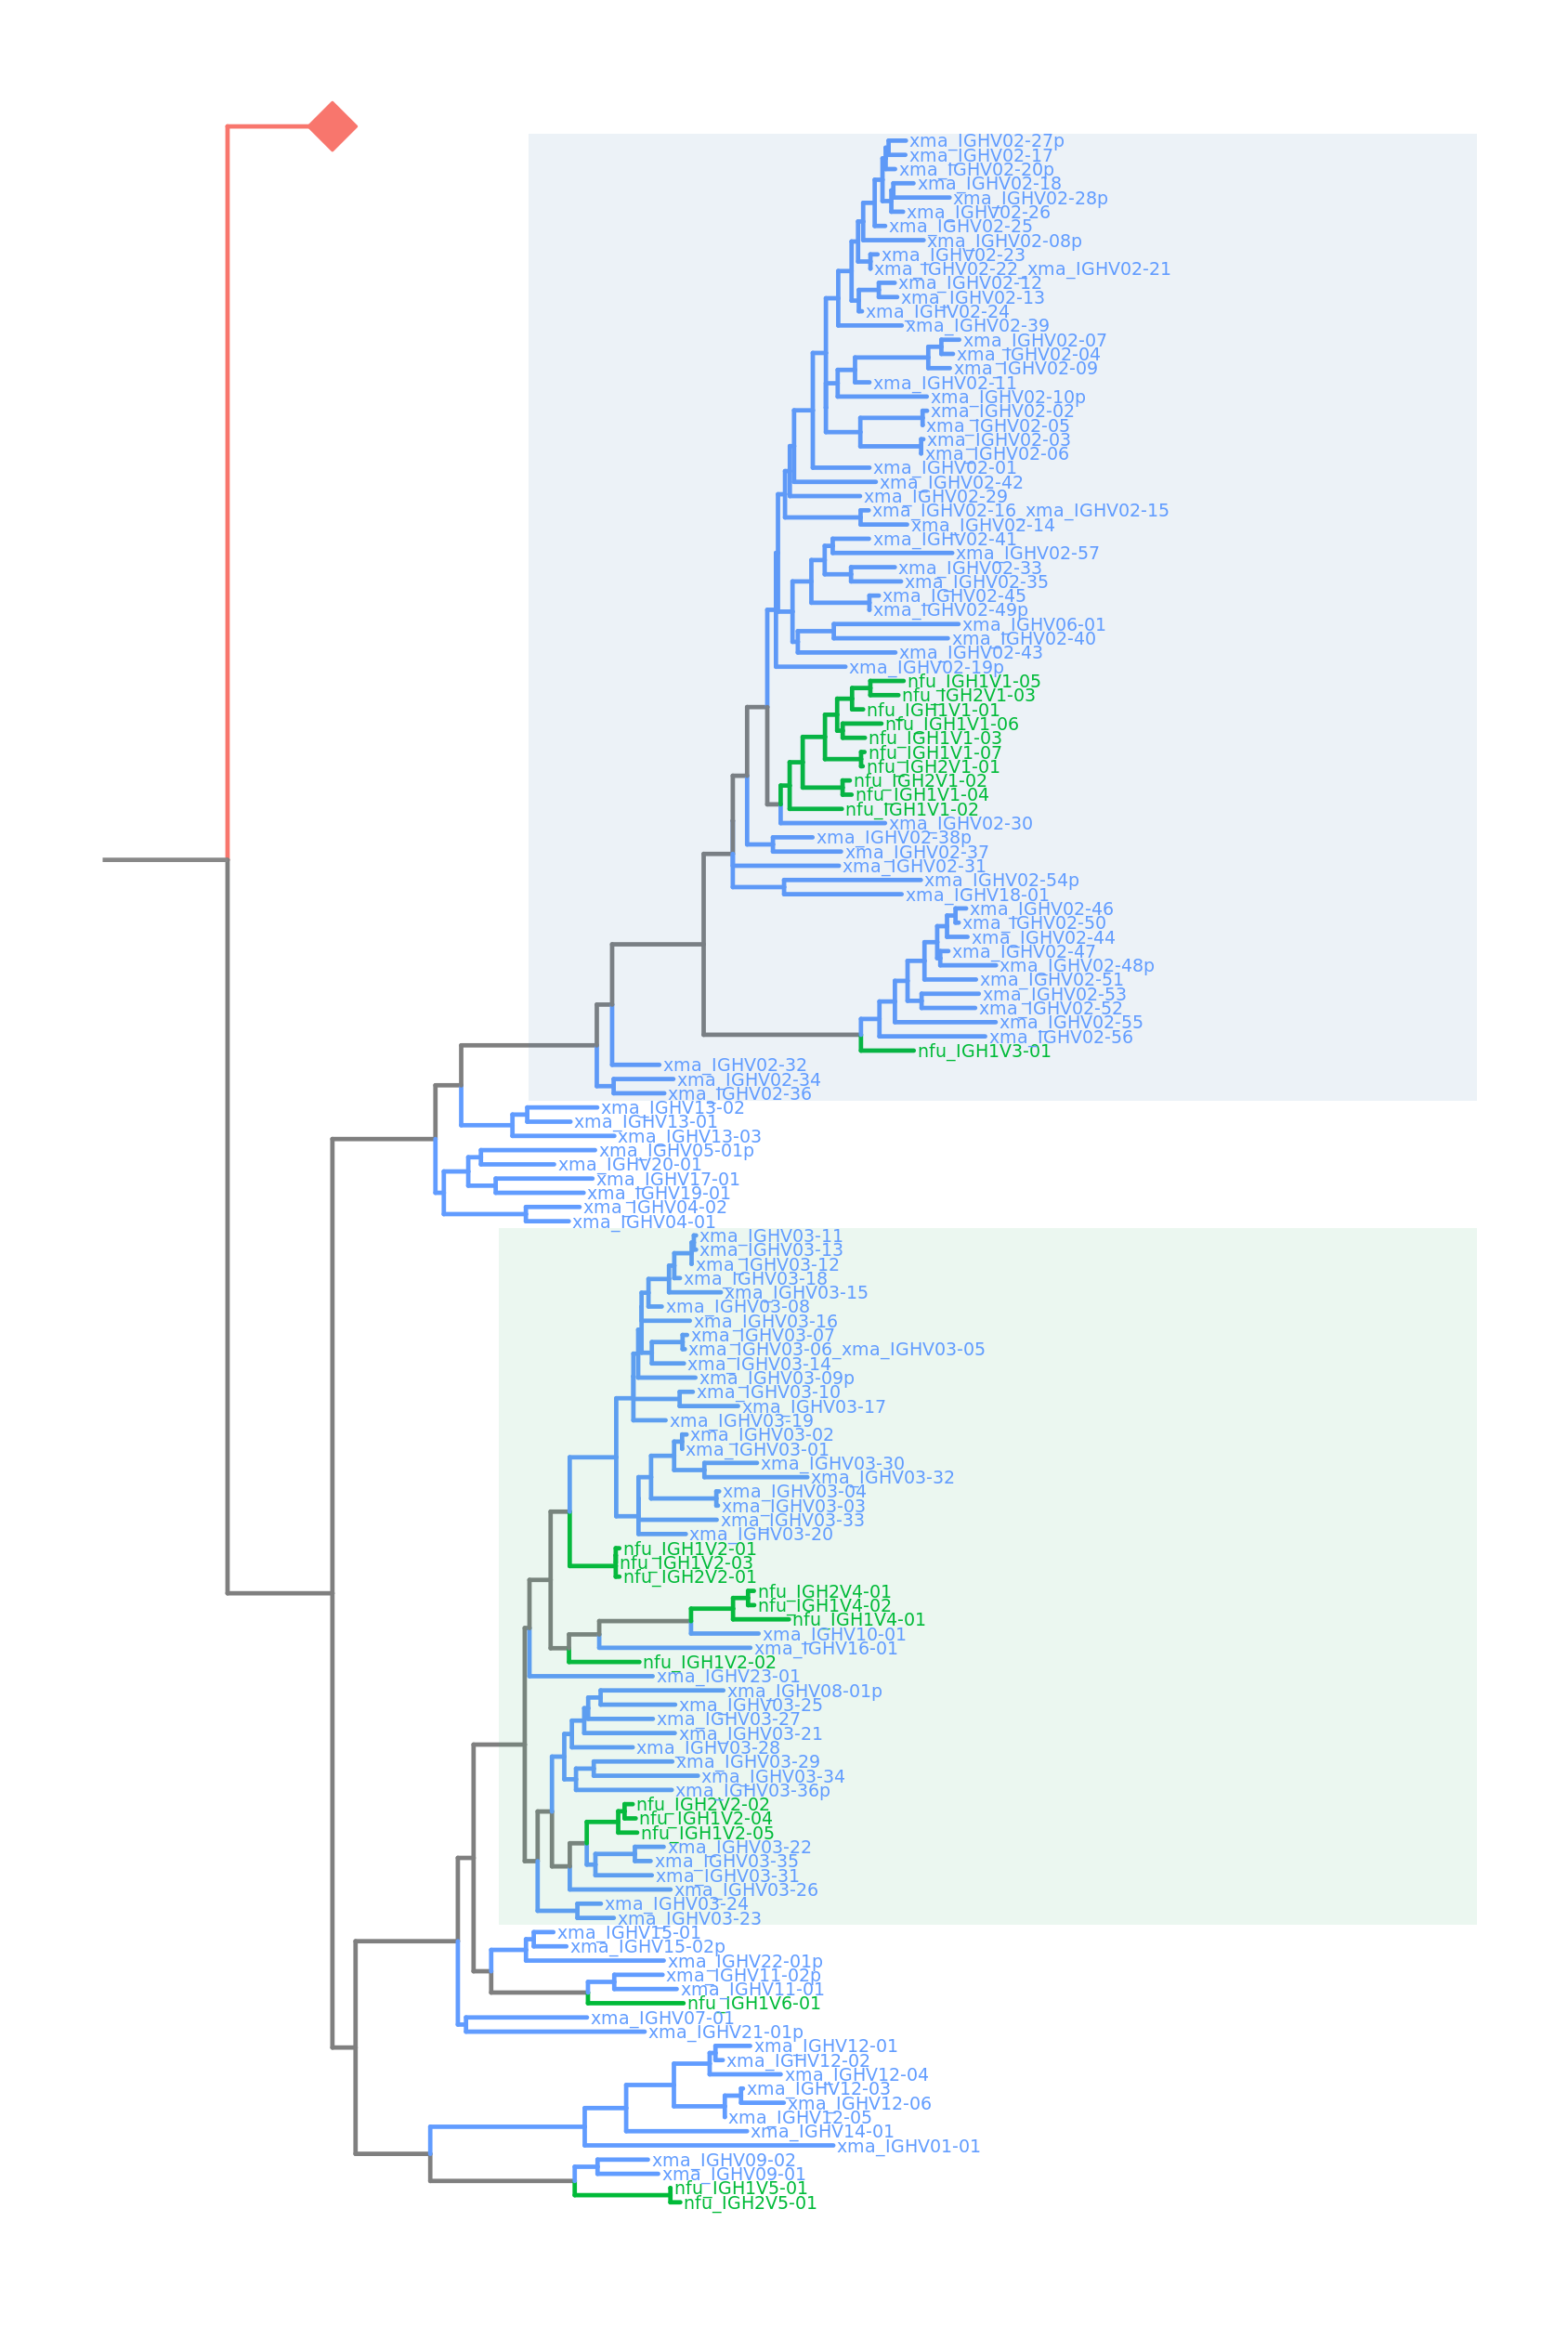
\includegraphics[width=0.8\textwidth]{_Figures/png/nfu-xma-vh-tree-nt.png}
	\caption[Evolutionary relationships between \vh families in \Xma and \Nfu]{\textbf{Evolutionary relationships between \vh families in \Xma and \Nfu:} Phylogenetic tree of evolutionary relationships between \textit{IGH} \vh segments in \Nfu and \Xma, as inferred from the nucleotide sequences of \vh segments from both loci. Note the close interrelationship between the largest (blue zone) and second-largest (green zone) families in each species. The red diamond indicates the location of the outgroup, which is composed of zebrafish \textit{TRB} V-segments.}
	\label{fig:nfu-xma-vh-tree-nt}
	\end{figure}
		
\FloatBarrier

\clearpage